\documentclass[10pt]{standalone}
\usepackage[utf8]{inputenc}
\usepackage{pgf,tikz }
%\pgfplotsset{compat=1.15}
\usepackage{mathrsfs}
\usetikzlibrary{arrows}
\pagestyle{empty}
\begin{document}

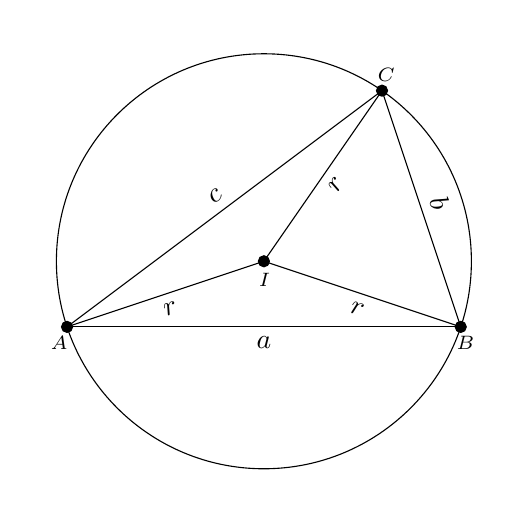
\begin{tikzpicture}[line cap=round,line join=round,>=triangle 45,x=1.0cm,y=1.0cm]

\clip(-0.5,-2.) rectangle (5.5,3.8);
\draw  (0.,0.)-- (4.,3.)node[pos=0.5, sloped,above] {$c$};
\draw  (4.,3.)-- (5.,0.)node[pos=0.5, sloped,above] {$b$};
\draw  (5.,0.)-- (0.,0.)node[pos=0.5, sloped,below] {$a$};
\draw  (2.5,0.8333333333333334) circle (2.6352313834736494cm);
\draw  (2.5,0.8333333333333334)-- (5.,0.)node[pos=0.5, sloped,below] {$r$};
\draw  (2.5,0.8333333333333334)-- (4.,3.)node[pos=0.5, sloped,below] {$r$};
\draw  (2.5,0.8333333333333334)-- (0.,0.)node[pos=0.5, sloped,below] {$r$};
\begin{scriptsize}
\draw [fill=black] (0.,0.) circle (2.0pt);
\draw (-0.1,-0.2) node {$A$};
\draw [fill=black] (5.,0.) circle (2.0pt);
\draw (5.05850133106587,-0.2) node {$B$};
\draw [fill=black] (4.,3.) circle (2.0pt);
\draw (4.053951751462685,3.2) node {$C$};
\draw [fill=black] (2.5,0.8333333333333334) circle (2.0pt);
\draw (2.5072643035022226,0.6) node {$I$};

\end{scriptsize}

\end{tikzpicture}
\end{document}